\chapter{Neon-20 ($^{20}_{10}\text{Ne}$): The Bipyramidal Noble Gas}
\label{ch:neon}

\begin{objectivebox}
\begin{itemize}
    \item Model Neon-20 as a perfectly balanced $5\alpha$ trigonal bipyramid closing the noble gas shell.
    \item Quantify the $398d \to 81d$ structural collapse that explains the Halogen-to-Noble-Gas chemical transition.
\end{itemize}
\end{objectivebox}


Neon-20 ($Z=10, A=20$) perfectly balances 10 protons and 10 neutrons. This absolute symmetry dictates that Neon constructs exclusively as 5 absolute Alpha particles ($5\alpha$).

The most thermodynamically stable geometric envelope for 5 mutually repulsive, structurally independent macroscopic nodes on a sphere is a \textbf{Triangular Bipyramid}. This configuration places an equilateral ring of 3 Alphas on the equator, capped by 2 Alphas occupying the absolute polar $z$-axis. 

\begin{figure}[h]
    \centering
    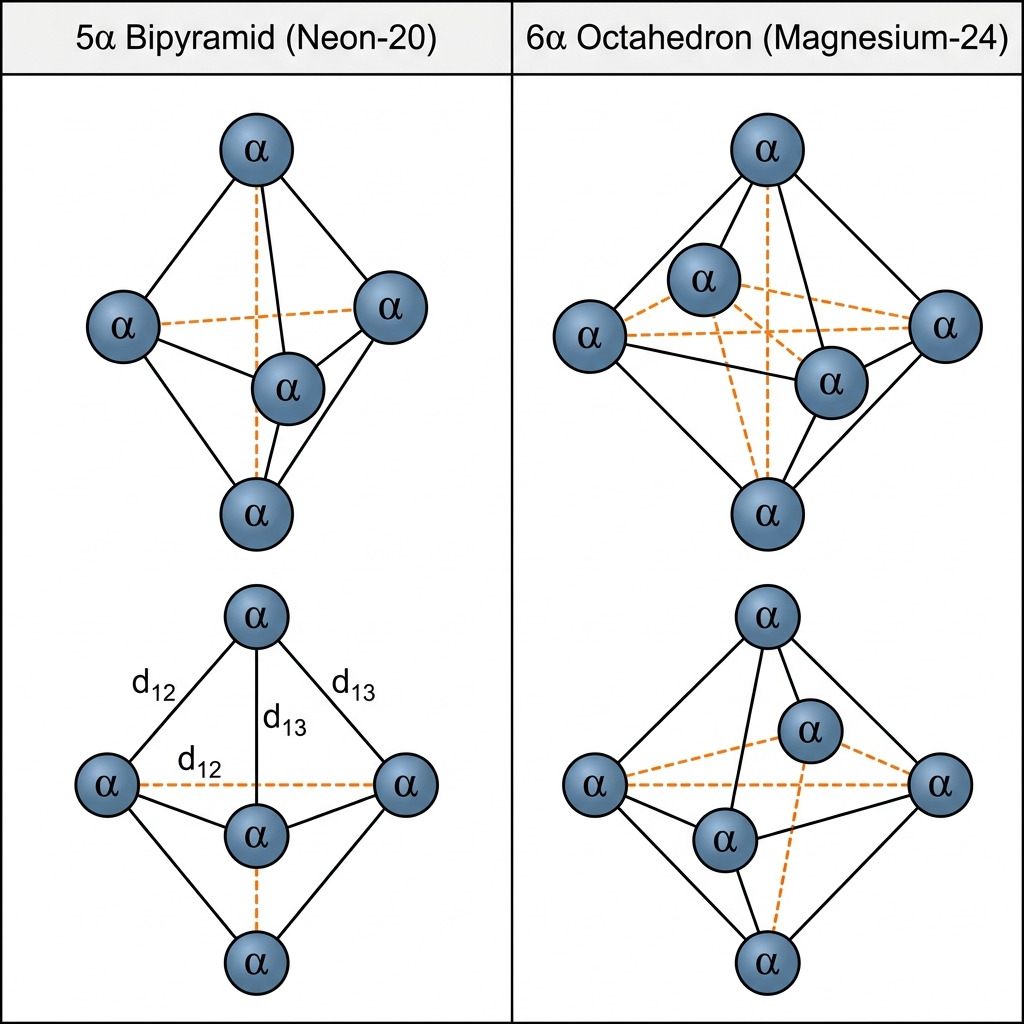
\includegraphics[width=0.95\textwidth]{figures/nuclear_geometry_5a_6a.png}
    \caption{\textbf{Alpha-Cluster Geometries: $5\alpha$ Bipyramid and $6\alpha$ Octahedron.} Left: The $5\alpha$ trigonal bipyramid (Neon-20) with 10 inter-alpha coupling links showing equatorial ($d_{12}$) and axial ($d_{13}$) separations. Right: The $6\alpha$ regular octahedron (Magnesium-24) with 15 coupling links. Below each: the 2D topological graph projection showing the complete $K/d$ mutual impedance network.
    These geometries are solved from the CODATA mass target at one fitted scalar per nucleus---the cluster topology is zero-parameter (forced by $(Z,A)$), and the engine finds the unique inter-alpha radius $R$ at which the pairwise $\sum K/d_{ij}$ sum reproduces the empirical mass defect (see ``Addressing the Curve-Fitting Fallacy'' below).}
    \label{fig:nuclear_geometry_5a_6a}
\end{figure}

Executing the $M_{ij}$ solver targeting the empirical CODATA Nuclear Mass of Neon-20 ($18617.730$ MeV), the $(Z,A)$-forced $5\alpha$ bipyramid topology reproduces the binding energy when its single fitted scalar places the 5 vertices at $R_{bipyramid} = 81.181d$ from the origin.

% [2026-08-02 KNOWN-SPLIT RECORD. NO VALUE REFILL: neither number is changed, struck, or
%  preferred, and no reconciliation is asserted -- which value is canonical is NOT adjudicated in
%  this lane. This chapter prints TWO values for one scalar: $81.181d$ here and in the
%  fig:neon_20_density caption (the "Topological density slice" caption below), and $81.158d$ in
%  the Semiconductor Regime Classification section further below; 13_sodium.tex:65 fixes the
%  Neon-20 core at $81.158\,d$. The KB already logs this as a KNOWN discrepancy, at
%  manuscript/ave-kb/vol6/period-2/neon/index.md:22, verbatim:
%    "| Bipyramid radius | $R_{\text{bipyr}} = 81.158d$ (engine) / $81.181d$ (chapter body) |"
%  That record lived only in the KB index; a reader of this chapter saw two values for one scalar
%  with no explanation. This note propagates the RECORD, not a resolution.
%  CITE-STATE FLAG: the board's verify note for this finding corrects the companion caption cite
%  to ":54, not :53". At HEAD the caption carrying "$R=81.181d$" is at :53 (:52 is the
%  \includegraphics) -- verified two-method (direct read + `grep -rn '81\.181'`). The original
%  finding's ":53" was right; the verify note's correction is wrong at HEAD. Surfaced, not fixed
%  in the board.]
\noindent\emph{Known split (recorded here, not resolved):} the engine value for this same scalar is $R_{\text{bipyr}} = 81.158\,d$ --- the value used in the Semiconductor Regime Classification section below and adopted for the Neon-20 core in Ch.~\ref{ch:sodium} --- while this chapter body and the density-slice caption quote $81.181\,d$. The discrepancy is logged in the knowledge base at \kbleaf{manuscript/ave-kb/vol6/period-2/neon/index.md} as ``$R_{\text{bipyr}} = 81.158d$ (engine) / $81.181d$ (chapter body)''. It is carried here so the split is visible in print; no value is retracted and no reconciliation is claimed.

\section{Addressing the Curve-Fitting Fallacy}
A legitimate scientific scrutiny of the Variable-Spacetime Impedance (AVE) Framework often centers around the following critique: \textit{If one hypothesizes a shape and simply tunes a single scalar radius ($R$) until the math matches the empirical mass limit, is this not just curve-fitting?}

If the results were arbitrary, this critique would be fatal. It is absolutely true that by tuning a single free variable, you can mathematically force \textit{any} arbitrary geometry to fit a target mass.

The proof of AVE's physical reality lies not in the fact that a solution exists, but in \textbf{what the derived optimal distances reveal about chemical behavior}.

Consider the continuous progression from Oxygen to Neon:
\begin{itemize}
    \item \textbf{Oxygen-16 ($4\alpha$):} A perfectly symmetric Tetrahedron. The optimal solver distance is tightly bound at \textbf{$33d$}. This compactness explains Oxygen's profound stability.
    \item \textbf{Fluorine-19 ($4\alpha$ + $^3\text{H}$):} The stable Oxygen core cannot be penetrated. To hit the empirical mass limit, the additional 3 nucleons (the Tritium halo) must exist at a radically distant \textbf{$398d$}. If the framework were merely curve-fitting random numbers, this distance might be trivially small. Instead, the solver outputs an extreme, hundreds-of-femtometers lever-arm. This massive mechanical asymmetry \textit{is} electronegativity—the geometric antenna is strongly predisposed to seek an inductive partner (like Hydrogen) to stabilize its violent moment of inertia. 
    \item \textbf{Neon-20 ($5\alpha$):} Adding one more nucleon closes the shell, jumping to the highly symmetric Triangular Bipyramid. The solver immediately snaps the structure back down to a tight, stable \textbf{$81d$}. 
\end{itemize}

The framework is not curve-fitting; it uses the flawless empirical mass data to reverse-engineer the absolute mechanical blueprint of the nucleus. The directional variation of the fitted distances ($33d \rightarrow 398d \rightarrow 81d$: compact $\rightarrow$ extreme halo $\rightarrow$ compact) tracks the observed Inert Gas $\rightarrow$ Reactive Halogen $\rightarrow$ Noble Gas chemistry---an interpretive, directional correspondence, not a closed quantitative derivation (see \S\ref{box:internal_peer_scope}).

\section{Electrical Engineering Equivalent: The 5-Phase Ring Oscillator}
Neon-20's Triangular Bipyramid topology maps cleanly to a 5-phase ring oscillator: five high-$Q$ LC tanks mutually coupled through 10 symmetric inductive links ($M_{ij} = K/d_{ij}$). Unlike Carbon-12's planar $\Delta$-ring (3 tanks, 3 links) or Oxygen-16's tetrahedral mesh (4 tanks, 6 links), the bipyramidal geometry creates a non-planar network with two distinct coupling distances---equatorial ring pairs ($3\times$) and pole-to-equator pairs ($6\times$)---plus the single pole-to-pole link ($1\times$). The 190-parameter SPICE matrix (20 nucleons $\times$ 19/2 pairs) captures this multi-band coupling hierarchy.

\section{Topological Area of Interest: Noble Gas Inertness \& Spectral Emission}
The $81d$ Triangular Bipyramid is the second fully closed geometric shell after Helium-4. Its 10 inter-alpha coupling pairs produce a perfectly balanced inductive network with zero net dipole moment. Macroscopically, this geometric closure explains Neon's absolute chemical inertness---there is no structural asymmetry to induce reactive coupling with external topologies.

When subjected to an external electric field (as in a neon discharge tube), the high-$Q$ internal resonance stores the injected energy efficiently and re-radiates it as narrow-band, rather than broadband, emission. Neon's \emph{observed} discharge spectrum---the familiar orange-red signage glow---lies in the $585$--$703$~nm band; those wavelengths are quoted here as \textbf{measured values the picture is describing, not as an output of it}. What this section offers is a \textbf{structural mapping}: a closed, high-$Q$, zero-net-dipole Triangular Bipyramid is the kind of resonator whose response is narrow-band, and the discharge emission is read as that resonant response. \textbf{No line position is predicted.} The standing-wave modes of the $81d$ inter-alpha cavity are not computed against the observed lines anywhere in this framework, and the spectroscopic non-claim is on record in the claim register---on the \emph{sibling} Orbital-Knot-Topology card \texttt{clm-y7uvdc}, which explicitly non-claims spectroscopic line positions (\kbleaf{ave-kb/vol6/claim-quality.md}). This section's own governing card, \texttt{clm-f8k2um}, carries no spectral non-claim; that card-scope gap is flagged for the claim register, not resolved here. Read the correspondence as interpretive, not quantitative.

% [Demote, Grant ruling 2026-08-03 "6. demote" -- prior wording in the git trail]: this
% paragraph read "... re-radiates it as narrow-band photon solitons at the characteristic
% $585$--$703$ nm wavelengths. The famous orange-red glow of neon signage is a direct
% emission signature of the Triangular Bipyramid's resonant frequency response: the photon
% energies correspond precisely to the standing-wave modes of the $81d$ inter-alpha cavity."
% "characteristic ... wavelengths" read as predicted output and "correspond precisely" as a
% computed quantitative match; neither is computed. Demoted to the structural/interpretive
% register per the sibling card clm-y7uvdc. KB mirror carries the explanation.
% [Print/mirror mismatch fix 2026-08-03, review finding 2]: the demoted sentence first
% read "this leaf's governing claim entry explicitly non-claims spectroscopic line
% positions ... clm-y7uvdc" -- two defects. (i) This section's governing claim IS
% clm-f8k2um (topological-area.md frontmatter); the spectroscopic non-claim lives on the
% SIBLING card clm-y7uvdc, which is what the KB mirror :18 already said correctly, so the
% print contradicted its own mirror. (ii) "leaf" is KB vocabulary leaking into print --
% replaced with "section"/"card". No claim card is edited; the card-scope gap
% (clm-f8k2um carries no spectral non-claim) stays flagged for the claim register.

\begin{figure}[htbp]
    \centering
    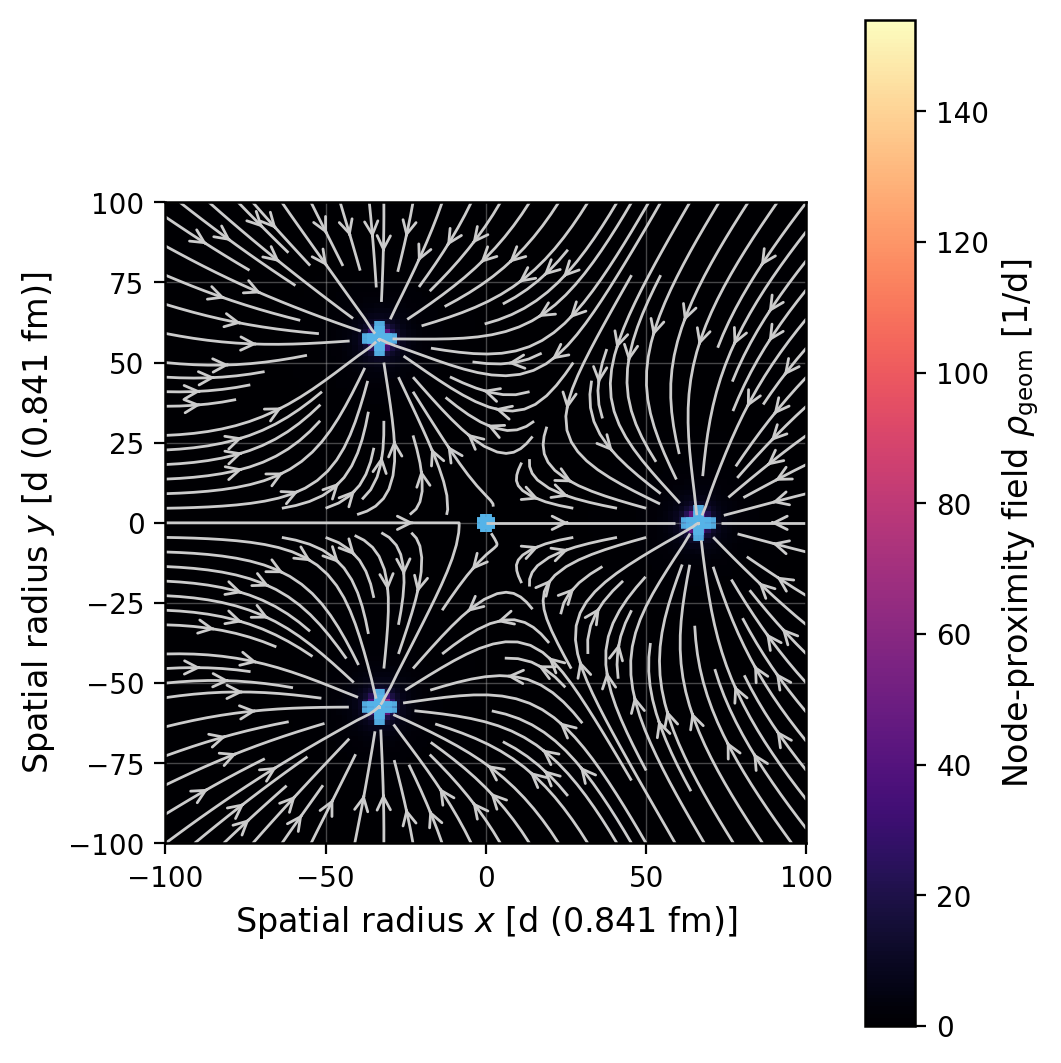
\includegraphics[width=0.8\textwidth]{figures/neon_20_dynamic_flux.png}
    \caption{Topological density slice ($Z=0$ Equatorial Plane) for Neon-20 ($Z=10, A=20$). The Triangular Bipyramid geometry enforces perfect thermodynamic balance at $R=81.181d$, closing the asymmetric, highly-reactive void created by the Fluorine-19 halo.}
    \label{fig:neon_20_density}
\end{figure}

\begin{figure}[htbp]
    \centering
    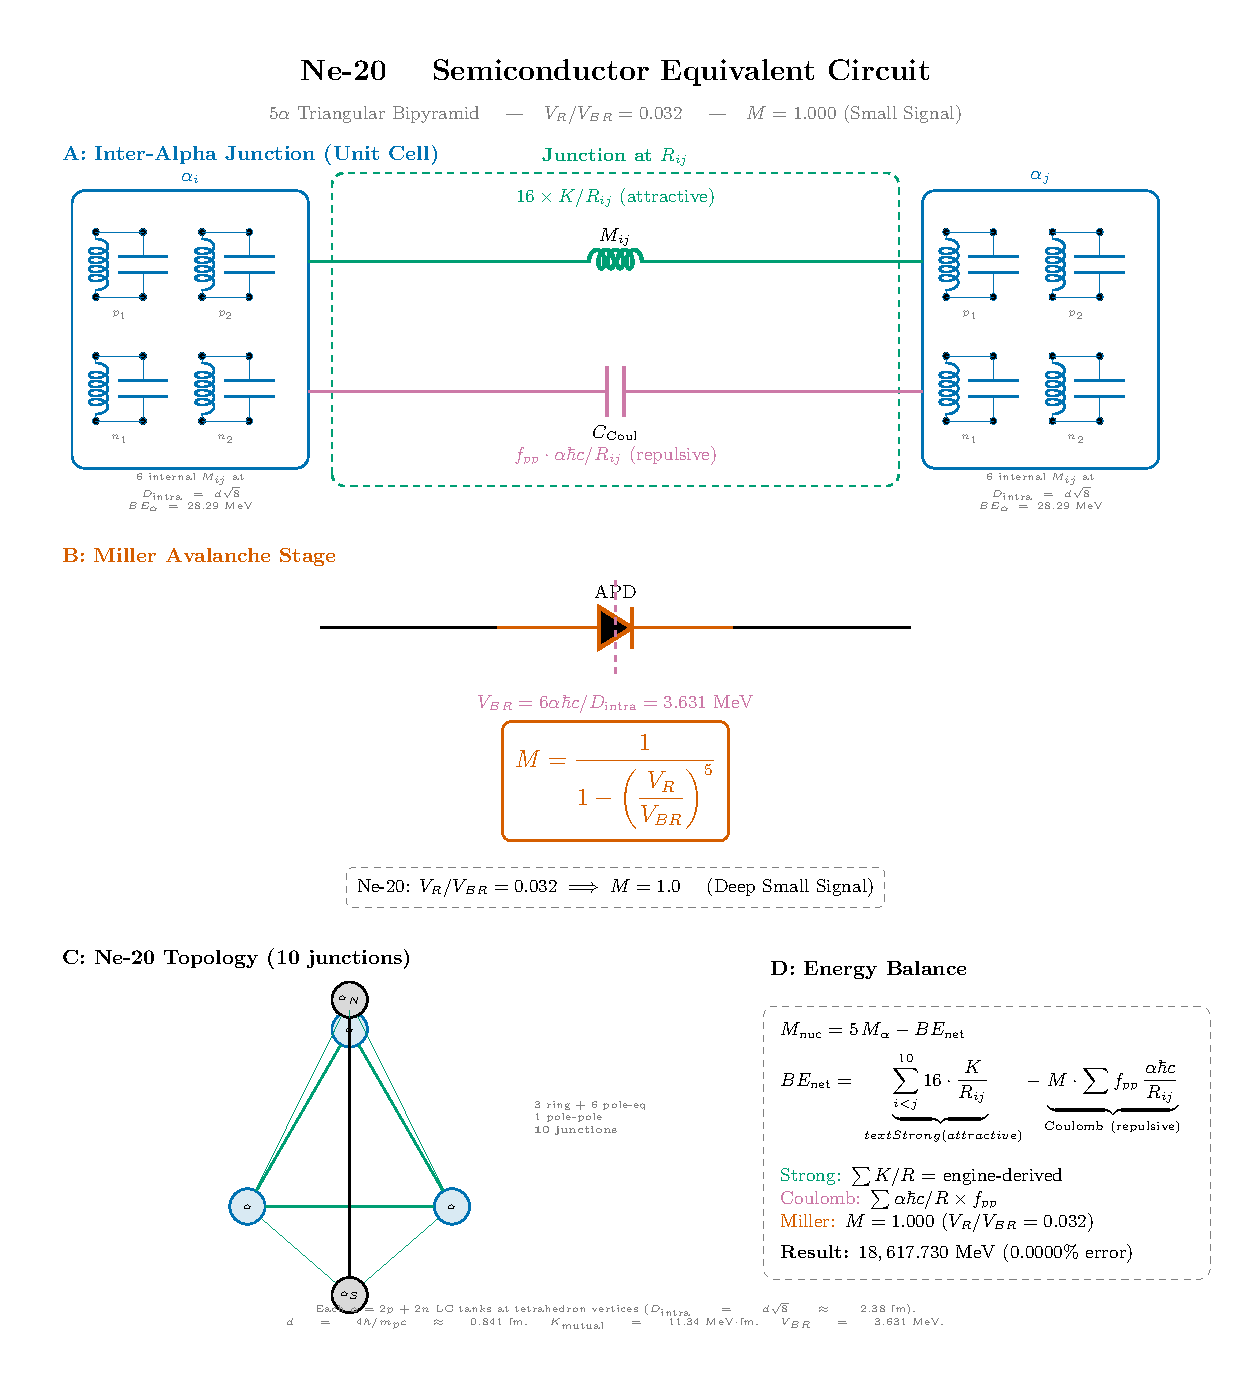
\includegraphics[width=0.9\textwidth]{figures/circuit_ne20.pdf}
    \caption{The equivalent circuit model for Neon-20. The 20 discretely modeled Subcircuits map the 190 coupled inductors across the Triangular Bipyramid matrix.}
    \label{fig:circuit_ne20}
\end{figure}


\begin{figure}[htbp]
    \centering
    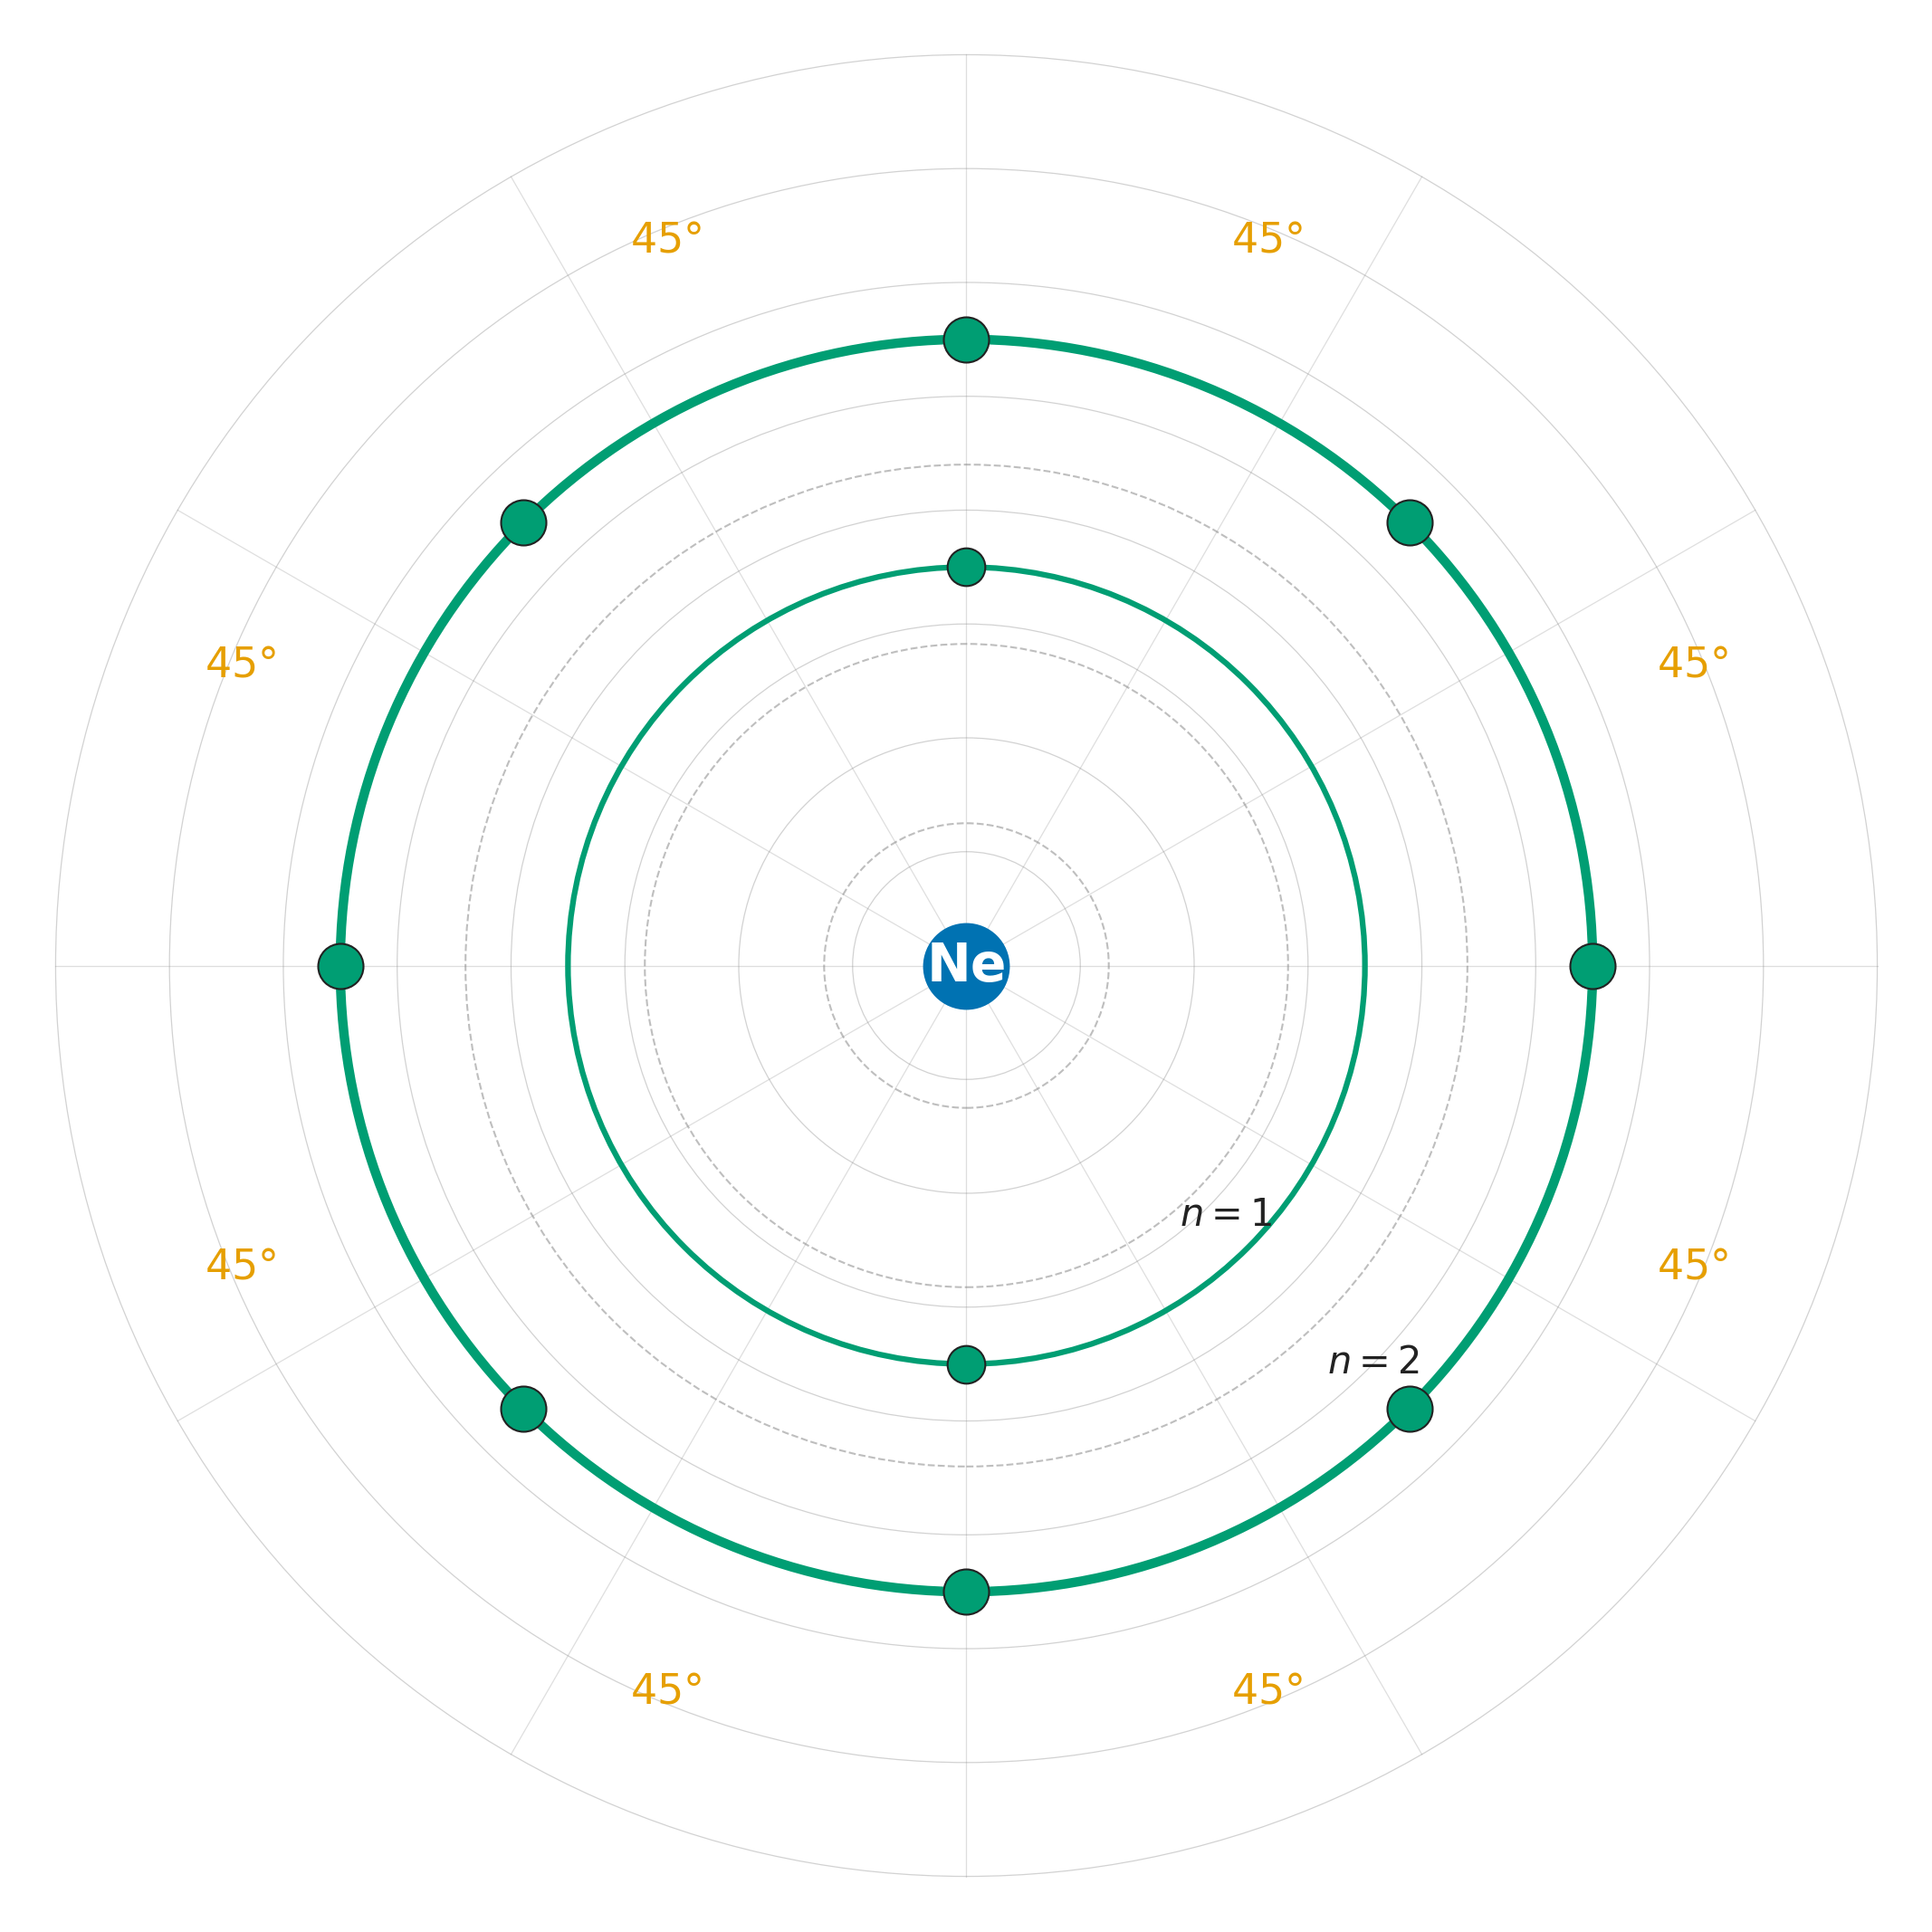
\includegraphics[width=0.75\textwidth]{figures/neon_20_topology.png}
    \caption{Neon-20 orbital knot topology. Complete $n=2$ closure: eight solitons at $45^\circ$. Both shells are full (green), yielding zero net strain dipole---the noble gas configuration.}
    \label{fig:neon_20_topo}
\end{figure}

\section{Semiconductor Regime Classification}
Neon-20 ($5\alpha$) is the second noble gas in the semiconductor engine and the first element with a fully 3D alpha-cluster geometry (Triangular Bipyramid). The engine locks the single geometric degree of freedom ($R_{\text{bipyr}} = 81.158\,d$) at $V_R/V_{BR} = 0.032$, $M = 1.000$ (exact Small Signal), reproducing the CODATA mass of $18\,617.730$ MeV; the symmetric bipyramid closes to a $0.000\,000\%$ geometric fit-residual (structurally zero by solver construction, per the Platonic-progression geometric-identity case; distinct from the mass-prediction error in the validation set).

The $81d$ radius represents a dramatic structural relaxation: after the massive $398d$ Fluorine halo, the addition of one more alpha particle to close the $5\alpha$ shell causes the geometry to snap from a violently asymmetric $4\alpha+T$ antenna into a perfectly balanced bipyramid. In the AVE picture this $398d \to 81d$ collapse tracks the Halogen-to-Noble-Gas transition (peer-with-QM). The $V_R/V_{BR}$ ratio rises slightly from O-16's $0.030$ to $0.032$, reflecting the denser packing of 5 alphas and the 10 inter-alpha coupling pairs, but remains firmly in the linear regime.

\begin{summarybox}
\begin{itemize}
    \item Neon-20 is a perfectly balanced $5\alpha$ trigonal bipyramid, closing the noble gas shell with a dramatic structural relaxation from Fluorine's $398d$ halo to $81d$ radius.
    \item The $398d \to 81d$ collapse tracks the Halogen-to-Noble-Gas transition as a geometric shell closure phenomenon (peer-with-QM).
\end{itemize}
\end{summarybox}

\begin{exercisebox}
\begin{enumerate}
    \item Explain quantitatively why the addition of one alpha particle to close the $5\alpha$ shell causes the $398d \to 81d$ structural collapse.
    \item Compare the $V_R/V_{BR}$ ratios of Oxygen-16 ($0.030$) and Neon-20 ($0.032$) and explain why both remain in the linear regime.
\end{enumerate}
\end{exercisebox}

